% File: anss2013-cotterell-medina.tex
% Author: Terrance Medina and Michael Cotterell
%
\documentclass[letterpaper,twocolumn,12pt]{article}
\usepackage[utf8]{inputenc}
\usepackage[english]{babel}
\usepackage{graphicx}
\usepackage{epsf}
\usepackage{rotating}
\usepackage{afterpage}
\usepackage{scs}
\usepackage{amsmath,amsfonts,amssymb,amsthm}
\usepackage{epsfig,epstopdf}
\usepackage{hyperref}
\usepackage{tkz-graph}
%\usepackage{citesort}

\usetikzlibrary{arrows}

\renewcommand\thesection{\arabic{section}}

\renewcommand{\topfraction}{0.95}
\renewcommand{\bottomfraction}{0.95}
\renewcommand{\textfraction}{0.05}
\renewcommand{\floatpagefraction}{0.35}

\begin{document}

\newtheorem{defn}{Definition}

\title{A Markov Model for Ontology Alignment}

\author{Michael E. Cotterell and Terrance Medina \\
Department of Computer Science \\
The University of Georgia \\
Athens, GA 30602-7404 \\
mepcott@uga.edu, medinat@uga.edu
}

\maketitle

\begin{abstract}
Ontology Alignment -- problem importance

Need for a way to determine convergence.

How does a Markov chain perform analytically?

\end{abstract}


\section{Introduction}

%\begin{itemize}
%\item Normalized Levenshtein Disance~\cite{yujian:2007:levenshtein}. 
%\item Similarity Flooding~\cite{melnik:2002:similarity}.
%\item Probability and Computing book~\cite{mitzenmacher:2005:probability}.
%\item Information-Theoretic~\cite{lin:1998:information}.
%\item Hungarian algorithm~\cite{kuhn:1955:hungarian}.
%\item Ontology Matching book~\cite{euzenat:2007:ontology}.
%\item ScalaTion~\cite{miller:2010:scalation}.
%\item BCNN book~\cite{bcnn:2010:simulation}.
%\item Scala spec~\cite{odersky:2011:spec}.
%\item My OEI paper~\cite{cotterell:2012:oei}.
%\item Linear Algebra textbook~\cite{goodaire:2003:linalgebra}.
%\item F-measure ref~\cite{rijsbergen:1979:ir}.
%\end{itemize}

As database technologies become increasingly diverse, the need to integrate those
technologies has become ever more important. The heterogeneous data problem
describes a common situation in which multiple data sources
with incompatible descriptions and data types must be integrated
for use by a single application. This problem is often encountered in 
the semantic web, which attempts to view the entire Internet as a unified database. 
A fundamental step in solving the heterogeneous data problem
is the production of an \textit{alignment} that can tell the client how to equate
the descriptions of two heterogeneous data sources.

An ontology alignment may be informally described as a set of correspondences 
between semantically related terms in two heterogeneous input ontologies. 
Each correspondence is qualified with a confidence level, $[0,1]$.
Alignment is useful in data integration tasks dealing with what is sometimes 
referred to as the semantic heterogeneity problem. 
It helps in the automation of various important tasks, most important of which 
is schema merging, enabling the knowledge and data expressed in the input 
ontologies to interoperate. \\

Ontology alignment algorithms are typically aggregations of multiple
basic techniques, which may be classified as lexical, symantic, structural etc. \cite{euzenat:2007:ontology}
In this paper, we consider the structural technique of
Similarity Flooding and present an improvement to that technique.

\noindent The rest of this paper is organized as follows: 
the remainder of this section will cover some of the background material related 
to the Semantic Web and ontologies, the cases for fully automated alignment, 
and some of the background material on the statistical methods used in this paper; 
Section~\ref{sec:approach} outlines the approach and implementation details; 
the evaluation and benchmarks are explained in Section~\ref{sec:eval}; 
results are presented in Section~\ref{sec:results}; and, 
conclusions and possible future work are outlined in Section~\ref{sec:conclusions}.

\subsection{Semantic Web and Ontologies}
\label{subsec:semanticweb}
First, we define some key terms around the Semantic Web and Ontology Alignment.

%Knowledge bases
A \textit{knowledge base} is a kind of database that is designed 
for decision support systems and expert systems. It specifically allows
machines to perform deductive reasoning over its elements.
For example, given the instance data ``John is a farmer'' and ``Farmers
wear overalls'', a knowledge base reasoner could deduce the new information
that ``John wears overalls''.

%KB representation
Knowledge bases (KBs) consist of \textit{entities} and
\textit{relations} between those entites. They are often represented as sets of
triples, that is, a set of two entities and a relationship between those
entities. For example, the triple ${\{teachers, lesson\_plans, write\}}$
defines the relationship that teachers write lesson\_plans.

%Ontologies
\textit{Ontologies} describe the relationships between elements in a knowledge base.
Similar to the notion of schemas in relational databases, ontologies specify
the structural relationships amongst the entities and classes of the ontology.

%Heterogeneous Data Problem
Frequently, queries must be performed across multiple knowledge bases. This is the
case when departments in a large enterprise maintain their own knowledge bases,
but must also share information with other departments. It is also a fundamental
requirement of the semantic web; users perform queries against the web,
and those queries must be performed against knowledge bases that may belong to 
entities on opposite sides of the globe. This leads us to the problem of heterogeneous
data. When knowledge bases are maintained by different organizations, the ontologies
used to describe them will usually be different. They will use different names
to describe similar or identical concepts, for instance, one ontology may keep track
of `cars' while another keeps track of `automobiles' and still another keeps track of 
`autoProducts'. In fact the list could go on and on.

%Ontology Alignnment
\textit{Ontology Alignment} is the process of equating two heterogeneous ontologies by
finding valid correspondences between their sets of elements. 
%
For instance, an alignment between an auto parts manufacturer and an auto dealership
might tell us with 85\% certainty that ``anti\_lock\_brakes'' and ``ABS'' represent
the same thing.

%Importance of Ontology Alignment
This is important because it allows a query management system to translate the terminology
of a user's query into the terminology used by many different ontologies and thereby
to query heterogeneous knowledge bases.

\subsection{Why do we need fully automated alignment?}
\label{subsec:automated}
Fully-automated alignment techniques, that is, ontology alignment performed without
any input or approval from a human user, represents the ideal scenario for many
of the use cases already discussed. For example, in a Semantic Web query, the details
of equating ontology elements across heterogeneous KBs should remain completely
invisible to the user, who simply wants to know the showtimes of movies in his or her
zip code, which star actors with a maximum Kevin-Bacon-Distance of three.
On the other hand, in an Enterprise Integration context much of the information to
be integrated is extremely domain specific and even organization specific, and possibly
only known by a handful of organization veterans. In such a case, a fully-automated
alignment process may not be entirely feasible.

In any case, fully-automated alignment is an as-yet-unobtained goal. In this paper
we present an improvement to Similarity Flooding, a structural alignment technique. However,
both the original algorithm and our improvement rely on comparison against an ideal
alignment, produced by a human, for evaluation of the quality of the alignment. For our
evaluation, we have used the SEALS automated testing platform, which subjects an algorithm
to a battery of alignment test, and produces \textit{precision} and \textit{recall} scores
based on a comparison of its results against an ideal alignment result.



\section{Related Work}

Although the problem of fully-automated ontology alignment is far from being solved,
there has been much work accomplished around fundamental techniques for element
matching and aggregation of those matching techniques.\cite{euzenat:2007:ontology}.
One class of approaches
attempts to find element matches based on the relative similarity or dissimilarity
of the actual labels given to those elements. Some examples of these string-matching 
techniques are the Jaro-Winkler measure, the Levenshtein Distance and latent semantic 
indexing.
%
While useful in many situations, string-based matching techniques suffer from a common 
shortcoming; similar real-world objects often have very dissimilar names. The words
``car'' and ``autombile'' provide a good example.

Another class of techniques makes use of outside resources as aids in the search for
good matches between elements. Such outside resources include dictionaries or taxonomies
such as the WordNet taxonomy. These classes of techniques attempt to produce correspondences
between elements that may likely refer to the same real-world objects, but that have very
dissimilar names, such as ``car'' and ``automobile''. Some examples of these semantic 
approaches include Information-theoretic similarity.
%
The use of outside taxonomies can greatly improve the quality of matching results,
but such outside resources are not always readily available.

Yet a third class of matching techniques attempts to exploit the structure of the ontology
itself. For example, Similarity Flooding \cite{melnik:2002:similarity} takes a directed graph representation of an 
ontology and uses neighbor relations between the elements to find matches correspondences
between them. The idea is that if two elements in heterogeneous ontologies are very similar,
then their neighboring elements should also be very similar.

The Similarity Flooding algorithm operates by producing a new graph that
represents relationships amongst the entities in each input ontology. The
algorithm first takes the cross-product of all nodes
in both ontologies, producing a single node in the result graph for each
pairing of nodes in the input ontologies. Edges in the result graph are 
produced if and only if the original nodes from the input ontologies
both shared an edge. This results in a \textit{Pairwise Connectivity Graph}.
Finally, weights are added to the edges such all outbound edges from a given
node have equal weight, and sum to one. The result is a \textit{Propagation Graph}.

Once the Propagation Graph has been generated, the similarity score of each node
is generated as follows: each node is assigned an arbitrary initial similarity
score which is refined through an iterative fixpoint computation. At each iteration
the new similarity is equal to the old similarity plus the weighted sum of
the similarity of all its neighbors in the propagation graph. This fixpoint
computation proceeds until the new similarity converges to a fixed value.
%
%Convergence Properties
Similarity flooding has been useful as a foundation in other structure-based
matching techniques such as anchor flooding,
but suffers from 
a few limitations. First, it requires that the edges of the edge-labeled graph 
representation have identically named labels. In the case that corresponding edge labels
do not have exactly the same name, but mean the same thing (for example ``hasA'' and ``has\_a'')
that information is completely lost to the flooding algorithm. 
%Explain Propagation graph

%Note: are we still doing this?
%--------------------------------
%It can also be difficult to predict
%wether or not the fixpoint calculation will converge.

\section{Approach \& Implementation}
%%%%%%%%%%% APPROACH & IMPLEMENTATION  %%%%%%%%%%%%%%%%%%%%%%%%%%%%%%%%%%%%%%%%
\label{sec:approach}

The following sections outline and present the details about the model as well as 
many of the implementation details.

\subsection{Levenshtein Edit Distance}
%%%%%%%%%%% LEVENSHTEIN DISTANCE  %%%%%%%%%%%%%%%%%%%%%%%%%%%%%%%%%%%%%%%%%%%%%%%%%%%%

The Levenshtein distance is a string similarity metric for measuring the difference 
between two character sequences. 
The distance between two sequences is equal to the number of single-character 
operations required to transform one sequence into the other. 
The single-character operations are insertion, deletion, and substitution.

\begin{defn}
Let $x$ and $y$ be terms in a single ontology. The label set $\Lambda \left( x, y \right)$ is the set of all labels between hierarchical properties and object properties where $x$ and $y$ are the domain and range of a property, respectively.
\end{defn}

\begin{figure*}
\centering
\begin{equation*}
\mathcal{L} 
\left( \alpha_i, \beta_j \right) = \left\{
	\begin{array}{ll}
   	 	0 &: i=j=0 \\
		i &: j = 0 \text{ and } i > 0 \\
		j &: i = 0 \text{ and } j > 0 \\
		\min 
			\left\{ 
			\begin{array}{l}
				\mathcal{L} \left( \alpha_{i-1}, \beta_j \right) + 1 \\
          		        \mathcal{L} \left( \alpha_i, \beta_{j-1} \right) + 1 \\
          		        \mathcal{L} \left( \alpha_{i-1}, \beta_{j-1} \right) + [\alpha_i \neq \beta_j]
			\end{array} \right. &: \text{else}
     \end{array}
\right.
\end{equation*}
\caption{Levenshtein Edit Distance}
\end{figure*}

\begin{figure*}
\centering
\begin{equation*}
\sigma
\left( \alpha_i, \beta_j \right) = \left\{
\begin{array}{ll}
  1           &: \mathcal{L} \left( \alpha_i, \beta_j \right) = 0 \\
  \frac{3}{4} &: \mathcal{L} \left( \alpha_i, \beta_j \right) = 1 \\
  \frac{1}{\mathcal{L} \left( \alpha_i, \beta_j \right)} &: \text{otherwise} \\
\end{array}
\right.
\end{equation*}
\caption{Edit Similarity Distance}
\end{figure*}

\subsection{Edge Confidence}
%%%%%%%%%%% EDGE CONFIDENCE %%%%%%%%%%%%%%%%%%%%%%%%%%%%%%%%%%%%%%%%%%%%%%%%%%%%
These lexical similarity techniques give us a way of assessing the 
similarity of two entities regardless of any structural relationships
they may have within an ontology. Recall that one limitation of the
Similarity Flooding technique is the necessity that predicates 
(edge labels when the ontology is represented as a graph) must have
names that correspond exactly. But this is an unrealistic requirement. 
It is easy to imagine that two unrelated ontologies might, for instance,
use predicates labeled ``appearsIn'' and ``actsIn'' to describe the
relationship that a certain actor has been in a movie (possibly with
Kevin Bacon).

We propose using lexical similarity to quantify a degree of similarity
between predicate levels. If the similarity is above some arbitrary
threshhold, we will consider the two predicates to mean the same thing.
In this way, we can include more edges in the propagation graph,
which provides more information about structural relationships to
the alignment algorithm.

Next we are faced with the problem of assigning an actual value to the
edge similarity. In the propagation graph for similarity flooding, each
outbound edge from a node is given the same weight as all of the other
edges from that node, and those weights all sum to one. This allows the 
graph to be described by a row-stochastic matrix. We would like to keep
that row-stochastic property for our edge confidence implementation, but 
we would also like to have different weights on each outbound edge,
proportionate to the degree of similarity (and thus the confidence) shared
by the ontology predicates represented by the edge in the propagation graph.

To this end, we start with a dissimilarity metric, such as one provided
by the Levenshtein distance algorithm. Next we derive a complement for this
weight by taking its difference from the sum of all outbound edge weights
for a particular node. Finally, the edge weight is given as the ratio of
that complement, and the sum of all complements for outbound edges of a
particular node.

This concept is formalized in the definitions that follow.

\begin{defn}
\label{edgeconfidence}
Let $\gamma$ be some threshold. Edge confidence $\Gamma \left( \alpha, \beta \right)$ is the similarity score between the labels of two edges $\alpha$ and $\beta$ if that similarity is greater than $\gamma$, otherwise $0$. That is,
$$ \Gamma \left( \alpha, \beta \right) = \left\{
   	 \begin{array}{ll}
           \frac{1}{\sigma \left( \alpha, \beta \right)} & : \vert \sigma \left( \alpha, \beta \right) \vert \geq \gamma \\
           0                                             & : \mathrm{otherwise}
     \end{array}
   \right.$$
\end{defn}

\subsection{Unnormalized Pairwise Markov Chain}
%%%%%%%%%%% UPMC %%%%%%%%%%%%%%%%%%%%%%%%%%%%%%%%%%%%%%%%%%%%%%%%%%%%%%%%%%%%%%
In the definitions that follow, consider the input ontologies 
presented in Figure~\ref{fig:input}.

A Markov Chain is a mathematical model that represents a system as a set of states
and a set of probabilistic transitions between those states. Most importantly, Markov 
processes adhere to the Markov Property, that is, a system's next state depends only
on its current state, and not on any of its previous states. In that sense, Markov
processes are called ``memoryless''.

\begin{defn}
An {\bf Unnormalized Pairwise Markov Chain} is a not-necessarily stochastic Markov Chain that satisfies the following property.
For every pairwise grouping of ontological terms between the two input ontologies, there exists a transition in the UPMC
$$ (x, y) \rightarrow (x', y') $$
with probability $\Gamma(\Lambda(x, y), \Lambda(x', y'))$ if and only if
\begin{itemize}
\item there exists an edge from $x$ to $x'$, and
\item there exists an edge from $y$ to $y'$.
\end{itemize}
\end{defn}

The creation of a UPMC creates a directed graph between pairs of concepts that relate 
pairs based on their structural similarity.
The idea is that a pair of concepts are more likely to be similar if they are structurally similar.
Each pair of ontological terms is connceted to other pairs of ontological terms via directed 
edges that are proportional to similarity of the edges that exist in the input ontologies. 

\begin{figure*}
\centering
\SetVertexNormal[
	Shape = circle,
    % FillColor = orange,
    LineWidth = 1pt
]
\SetUpEdge[
	lw = 1pt,
    color = orange,
    labelcolor = white
]
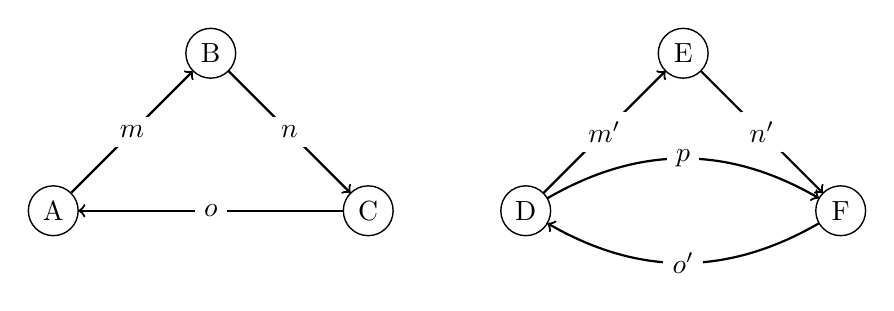
\begin{tikzpicture}
   \Vertex[x=0, y=0]{A}
   \Vertex[x=2, y=2]{B}
   \Vertex[x=4, y=0]{C}
   
   \Vertex[x=6, y=0]{D}
   \Vertex[x=8, y=2]{E}
   \Vertex[x=10, y=0]{F}
%   \tikzset{EdgeStyle/.append style = {bend left}}
   \tikzset{EdgeStyle/.style={->}}
   \Edge[label = $m$](A)(B)
   \Edge[label = $n$](B)(C)
   \Edge[label = $o$](C)(A)
   
   \Edge[label = $m'$](D)(E)
   \Edge[label = $n'$](E)(F)
   \tikzset{EdgeStyle/.append style = {bend left}}
   \Edge[label = $o'$](F)(D)
   \tikzset{EdgeStyle/.append style = {bend left}}
   \Edge[label = $p$](D)(F)  
\end{tikzpicture}
\caption{Example Input Ontologies with Object Properties}
\label{fig:input}
\end{figure*}

\begin{figure*}
\begin{equation*}
\left( \begin{array}{ccccccccc}
0 & b & c & a & a & a & a & a & a \\
d & 0 & f & a & a & a & a & a & a \\
g & h & 0 & a & a & a & a & a & a \\
g & h & i & 0 & a & a & a & a & a \\
g & h & i & j & 0 & a & a & a & a \\
g & h & 0 & a & a & 0 & a & a & a \\
g & h & 0 & a & a & a & 0 & a & a \\
g & h & 0 & a & a & a & a & 0 & a \\
g & h & 0 & a & a & a & a & a & 0 \end{array} \right)
\end{equation*}
\caption{Example an Unnormalized Pairwise Markov Chain}
\label{fig:upmc}
\end{figure*}

\subsection{Normalized Pairwise Markov Chain}

In order to take advantage of the convergance properties outlined earlier in this paper, the UPMC needs to have its probability transition matrix converted into a row stochastic form. 
This is done by normalizing the row sums of the matrix such that they sum to one.

\begin{defn}
\label{def:npmc}
a {\bf Normalized Pairwise Markov Chain (NPMC)} is defined as the Markov Chain generated from a UPMC by normalizing the row sums of the matrix such that they sum to one. Let $P$ be the $1$-step probability transition matrix for an UPMC. First, determine the sum of the current recipricol row sums.

$$ M_i = \sum \frac{1}{P_i} $$

\noindent Then, add the repricol row sums to each value in the matrix, storing each value in a temporary matrix $T$.

$$ T_{i,j} = -\frac{1}{P_{i,j}} + M_i $$

\noindent Normalize each value by dividing each value in $T$ by its row sum.

$$ P_{i,j} = \frac{T_{i,j}}{\sum T_i} $$
\end{defn}

\noindent The matrix that results from applying the transformation described in Definition~\ref{def:npmc} is \textit{row stochastic} (its rows sum to one).
When viewed as the $1$-step probability transition matrix for a Markov Chain, it is easy to see that the weights on the outgoing edges for each state sum to one.
After the transformation, a NPMC represents a Markov Chain where each pair of ontological terms has a certain probability of being related to other pairs in the chain in proportion to the edge confidences that were calculated earlier.

\subsection{Iterative Approach}

Once approach to finding the stationary distribution of the NPMC is to compute the limiting probabilistic state $\lim_{k \to \infty} \pi P^k$ in an iterative fashion. 
Let $\epsilon$ be some threshold.

$$ A = \pi^t : \pi^t P \pm \epsilon = \pi^{t-1} $$

\noindent The values for the initial similarity distribution $\pi^0$ are taken from the non-structural similarity scores for the ontological terms corresponding to each state.

\subsection{Steady-State Approach}

Another approach to finding the stationary distribution of the NPMC is to compute the limiting probabilistic state $\lim_{k \to \infty} \pi P^k$ directly.
This can be done by solving a left eigenvalue problem: 
$$ \pi = \pi P \Rightarrow \pi (P - I) = 0$$
where the eigenvalue is $1$ and $I$ is the identity matrix. 
Simply solve for $\pi$ by computing the left nullspace of the $P - I$ matrix (appropriately sliced) and then normalizing $\pi$ so that $\vert\vert \pi \vert\vert = 1$.
In order to accomplish this in an easy fashion, the ScalaTion library was used~\cite{miller:2010:scalation}.

\subsection{Refining Results}

The results generated from using either the iterative approach or the steady-state approach are only somewhat meaningful.
The ouput of both procedures produces a two-dimensional distribution of similarity scores between the two input ontologies.
Although this satisfies the definition of an alignment as presented earlier in this paper, a user is likely more interested in the set of similarities that yield the best correspondance between the two input ontologies.

Take the alignment distribution generated by either the iterative or steady-state approach and decompose it into an $m \times n$ matrix.
Consider this matrix to be representative of a weighted bipartite graph.
Now, finding the set of similarities that yield the best correspondance between the two ontologies is simply a matter of solving the maximum-weighted bipartite graph matching problem using the generated graph.
In order to accomplish this task, the Hungarian algorithm is used~\cite{kuhn:1955:hungarian}.


%\subsection{Implementation Details}
%NOTE: I don't think we need to go into this too much (TM)
%
%Talk about the implementation here..

\section{Evaluation}
\label{sec:eval}

In order to evaluate the model presented in this paper, the bibliographic ontology benchmark provided by the Ontology Alignment Evaluation Initiative (OAEI) was used.
This benchmark test library consists of data sets that are built from the bibliographic reference ontology.
Each test includes a reference alignment in order to facilitate the calculation of precision and recall.

In order to evaluate the ontology alignment models presented in this paper, the Semantic Evaluation At Large Scale (SEALS) Platform was used~\cite{esteban:2010:executing, wrigley:2010:evaluating}.
The SEALS Platform is an extensible infrastructure developed by INSERT that facilitates the remote evaluation of various semantic technologies.
In our evaluation, the SEALS Platform was used to easily compare the models presented in this paper using the OAEI benchmark.

\section{Results}
\label{sec:results}
We compared our Edge Confidence algorithm to the stock Similarity Flooding algorithm
using the SEALS Benchmark 1 version 2.0 suite of tests. The SEALS platform subjects
each algorithm to a battery of alignment tests, then compares the result alignment
generated by the algorithm to an ideal alignment, which is included as part of the suite.
For each alignment test, the platform produces scores for \textit{precision} and \textit{recall}.

Precision is defined (Def \ref{def:precision} as the ratio of the number of correct correspondences to the total number
of correspondences returned by the algorithm. It should be noted that precision is mainly
a penalty against false positives, with no penalty against false negatives. For example if there
were 100 valid correspondences between two ontologies, a given algorithm could returned only a single
correspondence and, if that correspondence were correct, would score a 100\% precision. 

\begin{defn}
\textbf{Precision}
\label{def:precision}
$$
	precision = \frac{|\{valid \} \cap  \{returned \}|}{|\{returned \}|}
$$
\end{defn}

The converse of the precision metric is the recall metric (Def \ref{def:recall}, which provides a penalty for 
false negatives, but not for false positives. Recall considers the ratio of the correct
correspondences to the total number of correspondences that should have been returned by
the algorithm.

\begin{defn}
\textbf{Recall}
\label{def:recall}
$$
	recall = \frac{|\{valid \} \cap  \{returned \}|}{|\{valid \}|}
$$
\end{defn}

Finally, we consider the F-measure (Def \ref{def:fmeasure}), a metric that provides a 
balance between precision and recall. 

\begin{defn}
				\textbf{F-measure}
\label{def:fmeasure}
$$
	F = 2*\frac{precision * recall}{precision + recall}	
$$
\end{defn}

When comparing Similarity Flooding and Edge Confidence on the basis of precision,
Similarity Flooding typically outperforms Edge Confidence, as can be seen in Figure
\ref{fig:precision}. This reflects the conservative nature of Similarity Flooding.
Because Edge Confidence is more aggressive about including edges, it generates a 
larger propagation graph, which leads to more correspondences on average, although
this will typically include more incorrect results, thus lowering the precision
score.

By the same reasoning, Edge Flooding typically outperforms Similarity Flooding
on the basis of recall. Because Edge Flooding return more results, it has more
correct results, which gives a higher recall score. This is evident in Figure \ref{fig:recall}.

The real question is: does the more aggressive approach pay off in the F-measure
score, or does it extract too much of a penalty because of its lack of precision?
Figure \ref{fig:fmeasure} shows that the Edge Flooding technique performs very
well against Similarity Flooding, performing orders of magnitude better on many of 
the tests.

\section{Conclusions \& Future Work}
\label{sec:conclusions}


Some possible work includes, but is not limitted to, the following:

\begin{itemize}
\item Tweak the definition of edge confidence so that it includes information about the structural relationships between different object properties.
For example, object properties have parent-child relationships similar to ontological terms.
A new edge confidence function could take advantage of these relationships in order to consider a more structural approach to the alignment problem.
\item Investigate the use of Eigenvalues to evaluate the convergence values of the propagation graph in constant time.
\item Investigate the use of the Hungarian Algorithm to improve the quality of edge confidence values.
\end{itemize}

%All of the source code for this project can be found at ...

%ACKNOWLEDGMENTS are optional
\section*{Acknowledgments}

We would like to acknowledge Dr. John Miller at the University of Georgia for providing us the opportunity to pursue this study through his Advanced Databases course. 

%\bibliographystyle{abbrvnat}
\bibliographystyle{abbrv}
\bibliography{refs} 

\section*{Author Biographies} 
\vspace{8 pt}
\noindent \textbf{MICHAEL E. COTTERELL} is a Ph.D. student in Computer Science at the University of Georgia. 
He received his B.S. in Computer Science from UGA in May 2011. 
As an undergraduate, he served as the Vice President of the UGA Chapter of the Association for Computer Machinery (ACM) for two years. 
He also interned at the National Renewable Energy Lab, where he conducted research on formal ontologies for Energy Systems Integration and the Energy Informatics domain. 
His research interests include Simulation, Optimization, Semantic Web and Domain-Specific Languages with inter-disciplinary applications related to both Bioinformatics and Energy Informatics.
His email address is \href{mailto:mepcott@uga.edu}{mepcott@uga.edu}.
His curriculum vitae and list of publications are available at \url{http://michaelcotterell.com/}.

\vspace{8 pt}
\noindent \textbf{TERRANCE MEDINA} is a Master's student in Computer Science at the University of Georiga.  
His research interests include Agent-based Modeling and Simulation, Computational Music and Robot Control Architectures.
His email address is \href{mailto:medinat@uga.edu}{medinat@uga.edu}.




\onecolumn
\begin{sidewaysfigure}
\centering
\tiny{% GNUPLOT: LaTeX picture with Postscript
\begingroup
  \makeatletter
  \providecommand\color[2][]{%
    \GenericError{(gnuplot) \space\space\space\@spaces}{%
      Package color not loaded in conjunction with
      terminal option `colourtext'%
    }{See the gnuplot documentation for explanation.%
    }{Either use 'blacktext' in gnuplot or load the package
      color.sty in LaTeX.}%
    \renewcommand\color[2][]{}%
  }%
  \providecommand\includegraphics[2][]{%
    \GenericError{(gnuplot) \space\space\space\@spaces}{%
      Package graphicx or graphics not loaded%
    }{See the gnuplot documentation for explanation.%
    }{The gnuplot epslatex terminal needs graphicx.sty or graphics.sty.}%
    \renewcommand\includegraphics[2][]{}%
  }%
  \providecommand\rotatebox[2]{#2}%
  \@ifundefined{ifGPcolor}{%
    \newif\ifGPcolor
    \GPcolortrue
  }{}%
  \@ifundefined{ifGPblacktext}{%
    \newif\ifGPblacktext
    \GPblacktexttrue
  }{}%
  % define a \g@addto@macro without @ in the name:
  \let\gplgaddtomacro\g@addto@macro
  % define empty templates for all commands taking text:
  \gdef\gplbacktext{}%
  \gdef\gplfronttext{}%
  \makeatother
  \ifGPblacktext
    % no textcolor at all
    \def\colorrgb#1{}%
    \def\colorgray#1{}%
  \else
    % gray or color?
    \ifGPcolor
      \def\colorrgb#1{\color[rgb]{#1}}%
      \def\colorgray#1{\color[gray]{#1}}%
      \expandafter\def\csname LTw\endcsname{\color{white}}%
      \expandafter\def\csname LTb\endcsname{\color{black}}%
      \expandafter\def\csname LTa\endcsname{\color{black}}%
      \expandafter\def\csname LT0\endcsname{\color[rgb]{1,0,0}}%
      \expandafter\def\csname LT1\endcsname{\color[rgb]{0,1,0}}%
      \expandafter\def\csname LT2\endcsname{\color[rgb]{0,0,1}}%
      \expandafter\def\csname LT3\endcsname{\color[rgb]{1,0,1}}%
      \expandafter\def\csname LT4\endcsname{\color[rgb]{0,1,1}}%
      \expandafter\def\csname LT5\endcsname{\color[rgb]{1,1,0}}%
      \expandafter\def\csname LT6\endcsname{\color[rgb]{0,0,0}}%
      \expandafter\def\csname LT7\endcsname{\color[rgb]{1,0.3,0}}%
      \expandafter\def\csname LT8\endcsname{\color[rgb]{0.5,0.5,0.5}}%
    \else
      % gray
      \def\colorrgb#1{\color{black}}%
      \def\colorgray#1{\color[gray]{#1}}%
      \expandafter\def\csname LTw\endcsname{\color{white}}%
      \expandafter\def\csname LTb\endcsname{\color{black}}%
      \expandafter\def\csname LTa\endcsname{\color{black}}%
      \expandafter\def\csname LT0\endcsname{\color{black}}%
      \expandafter\def\csname LT1\endcsname{\color{black}}%
      \expandafter\def\csname LT2\endcsname{\color{black}}%
      \expandafter\def\csname LT3\endcsname{\color{black}}%
      \expandafter\def\csname LT4\endcsname{\color{black}}%
      \expandafter\def\csname LT5\endcsname{\color{black}}%
      \expandafter\def\csname LT6\endcsname{\color{black}}%
      \expandafter\def\csname LT7\endcsname{\color{black}}%
      \expandafter\def\csname LT8\endcsname{\color{black}}%
    \fi
  \fi
  \setlength{\unitlength}{0.0500bp}%
  \begin{picture}(12960.00,9360.00)%
    \gplgaddtomacro\gplbacktext{%
      \csname LTb\endcsname%
      \put(946,1144){\makebox(0,0)[r]{\strut{} 0}}%
      \put(946,2611){\makebox(0,0)[r]{\strut{} 0.2}}%
      \put(946,4078){\makebox(0,0)[r]{\strut{} 0.4}}%
      \put(946,5545){\makebox(0,0)[r]{\strut{} 0.6}}%
      \put(946,7012){\makebox(0,0)[r]{\strut{} 0.8}}%
      \put(946,8479){\makebox(0,0)[r]{\strut{} 1}}%
      \put(1185,1078){\rotatebox{-90}{\makebox(0,0)[l]{\strut{}101}}}%
      \put(1293,1078){\rotatebox{-90}{\makebox(0,0)[l]{\strut{}103}}}%
      \put(1400,1078){\rotatebox{-90}{\makebox(0,0)[l]{\strut{}104}}}%
      \put(1507,1078){\rotatebox{-90}{\makebox(0,0)[l]{\strut{}201}}}%
      \put(1615,1078){\rotatebox{-90}{\makebox(0,0)[l]{\strut{}201-2}}}%
      \put(1722,1078){\rotatebox{-90}{\makebox(0,0)[l]{\strut{}201-4}}}%
      \put(1829,1078){\rotatebox{-90}{\makebox(0,0)[l]{\strut{}201-6}}}%
      \put(1937,1078){\rotatebox{-90}{\makebox(0,0)[l]{\strut{}201-8}}}%
      \put(2044,1078){\rotatebox{-90}{\makebox(0,0)[l]{\strut{}202}}}%
      \put(2151,1078){\rotatebox{-90}{\makebox(0,0)[l]{\strut{}202-2}}}%
      \put(2259,1078){\rotatebox{-90}{\makebox(0,0)[l]{\strut{}202-4}}}%
      \put(2366,1078){\rotatebox{-90}{\makebox(0,0)[l]{\strut{}202-6}}}%
      \put(2473,1078){\rotatebox{-90}{\makebox(0,0)[l]{\strut{}202-8}}}%
      \put(2581,1078){\rotatebox{-90}{\makebox(0,0)[l]{\strut{}203}}}%
      \put(2688,1078){\rotatebox{-90}{\makebox(0,0)[l]{\strut{}204}}}%
      \put(2795,1078){\rotatebox{-90}{\makebox(0,0)[l]{\strut{}205}}}%
      \put(2903,1078){\rotatebox{-90}{\makebox(0,0)[l]{\strut{}206}}}%
      \put(3010,1078){\rotatebox{-90}{\makebox(0,0)[l]{\strut{}207}}}%
      \put(3117,1078){\rotatebox{-90}{\makebox(0,0)[l]{\strut{}208}}}%
      \put(3225,1078){\rotatebox{-90}{\makebox(0,0)[l]{\strut{}209}}}%
      \put(3332,1078){\rotatebox{-90}{\makebox(0,0)[l]{\strut{}210}}}%
      \put(3439,1078){\rotatebox{-90}{\makebox(0,0)[l]{\strut{}221}}}%
      \put(3547,1078){\rotatebox{-90}{\makebox(0,0)[l]{\strut{}222}}}%
      \put(3654,1078){\rotatebox{-90}{\makebox(0,0)[l]{\strut{}223}}}%
      \put(3761,1078){\rotatebox{-90}{\makebox(0,0)[l]{\strut{}224}}}%
      \put(3869,1078){\rotatebox{-90}{\makebox(0,0)[l]{\strut{}225}}}%
      \put(3976,1078){\rotatebox{-90}{\makebox(0,0)[l]{\strut{}228}}}%
      \put(4083,1078){\rotatebox{-90}{\makebox(0,0)[l]{\strut{}230}}}%
      \put(4191,1078){\rotatebox{-90}{\makebox(0,0)[l]{\strut{}231}}}%
      \put(4298,1078){\rotatebox{-90}{\makebox(0,0)[l]{\strut{}232}}}%
      \put(4405,1078){\rotatebox{-90}{\makebox(0,0)[l]{\strut{}233}}}%
      \put(4513,1078){\rotatebox{-90}{\makebox(0,0)[l]{\strut{}236}}}%
      \put(4620,1078){\rotatebox{-90}{\makebox(0,0)[l]{\strut{}237}}}%
      \put(4727,1078){\rotatebox{-90}{\makebox(0,0)[l]{\strut{}238}}}%
      \put(4835,1078){\rotatebox{-90}{\makebox(0,0)[l]{\strut{}239}}}%
      \put(4942,1078){\rotatebox{-90}{\makebox(0,0)[l]{\strut{}240}}}%
      \put(5049,1078){\rotatebox{-90}{\makebox(0,0)[l]{\strut{}241}}}%
      \put(5157,1078){\rotatebox{-90}{\makebox(0,0)[l]{\strut{}246}}}%
      \put(5264,1078){\rotatebox{-90}{\makebox(0,0)[l]{\strut{}247}}}%
      \put(5371,1078){\rotatebox{-90}{\makebox(0,0)[l]{\strut{}248}}}%
      \put(5479,1078){\rotatebox{-90}{\makebox(0,0)[l]{\strut{}248-2}}}%
      \put(5586,1078){\rotatebox{-90}{\makebox(0,0)[l]{\strut{}248-4}}}%
      \put(5693,1078){\rotatebox{-90}{\makebox(0,0)[l]{\strut{}248-6}}}%
      \put(5801,1078){\rotatebox{-90}{\makebox(0,0)[l]{\strut{}248-8}}}%
      \put(5908,1078){\rotatebox{-90}{\makebox(0,0)[l]{\strut{}249}}}%
      \put(6015,1078){\rotatebox{-90}{\makebox(0,0)[l]{\strut{}249-2}}}%
      \put(6123,1078){\rotatebox{-90}{\makebox(0,0)[l]{\strut{}249-4}}}%
      \put(6230,1078){\rotatebox{-90}{\makebox(0,0)[l]{\strut{}249-6}}}%
      \put(6337,1078){\rotatebox{-90}{\makebox(0,0)[l]{\strut{}249-8}}}%
      \put(6445,1078){\rotatebox{-90}{\makebox(0,0)[l]{\strut{}250}}}%
      \put(6552,1078){\rotatebox{-90}{\makebox(0,0)[l]{\strut{}250-2}}}%
      \put(6659,1078){\rotatebox{-90}{\makebox(0,0)[l]{\strut{}250-4}}}%
      \put(6767,1078){\rotatebox{-90}{\makebox(0,0)[l]{\strut{}250-6}}}%
      \put(6874,1078){\rotatebox{-90}{\makebox(0,0)[l]{\strut{}250-8}}}%
      \put(6982,1078){\rotatebox{-90}{\makebox(0,0)[l]{\strut{}251}}}%
      \put(7089,1078){\rotatebox{-90}{\makebox(0,0)[l]{\strut{}251-2}}}%
      \put(7196,1078){\rotatebox{-90}{\makebox(0,0)[l]{\strut{}251-4}}}%
      \put(7304,1078){\rotatebox{-90}{\makebox(0,0)[l]{\strut{}251-6}}}%
      \put(7411,1078){\rotatebox{-90}{\makebox(0,0)[l]{\strut{}251-8}}}%
      \put(7518,1078){\rotatebox{-90}{\makebox(0,0)[l]{\strut{}252}}}%
      \put(7626,1078){\rotatebox{-90}{\makebox(0,0)[l]{\strut{}252-2}}}%
      \put(7733,1078){\rotatebox{-90}{\makebox(0,0)[l]{\strut{}252-4}}}%
      \put(7840,1078){\rotatebox{-90}{\makebox(0,0)[l]{\strut{}252-6}}}%
      \put(7948,1078){\rotatebox{-90}{\makebox(0,0)[l]{\strut{}252-8}}}%
      \put(8055,1078){\rotatebox{-90}{\makebox(0,0)[l]{\strut{}253}}}%
      \put(8162,1078){\rotatebox{-90}{\makebox(0,0)[l]{\strut{}253-2}}}%
      \put(8270,1078){\rotatebox{-90}{\makebox(0,0)[l]{\strut{}253-4}}}%
      \put(8377,1078){\rotatebox{-90}{\makebox(0,0)[l]{\strut{}253-6}}}%
      \put(8484,1078){\rotatebox{-90}{\makebox(0,0)[l]{\strut{}253-8}}}%
      \put(8592,1078){\rotatebox{-90}{\makebox(0,0)[l]{\strut{}254}}}%
      \put(8699,1078){\rotatebox{-90}{\makebox(0,0)[l]{\strut{}254-2}}}%
      \put(8806,1078){\rotatebox{-90}{\makebox(0,0)[l]{\strut{}254-4}}}%
      \put(8914,1078){\rotatebox{-90}{\makebox(0,0)[l]{\strut{}254-6}}}%
      \put(9021,1078){\rotatebox{-90}{\makebox(0,0)[l]{\strut{}254-8}}}%
      \put(9128,1078){\rotatebox{-90}{\makebox(0,0)[l]{\strut{}257}}}%
      \put(9236,1078){\rotatebox{-90}{\makebox(0,0)[l]{\strut{}257-2}}}%
      \put(9343,1078){\rotatebox{-90}{\makebox(0,0)[l]{\strut{}257-4}}}%
      \put(9450,1078){\rotatebox{-90}{\makebox(0,0)[l]{\strut{}257-6}}}%
      \put(9558,1078){\rotatebox{-90}{\makebox(0,0)[l]{\strut{}257-8}}}%
      \put(9665,1078){\rotatebox{-90}{\makebox(0,0)[l]{\strut{}258}}}%
      \put(9772,1078){\rotatebox{-90}{\makebox(0,0)[l]{\strut{}258-2}}}%
      \put(9880,1078){\rotatebox{-90}{\makebox(0,0)[l]{\strut{}258-4}}}%
      \put(9987,1078){\rotatebox{-90}{\makebox(0,0)[l]{\strut{}258-6}}}%
      \put(10094,1078){\rotatebox{-90}{\makebox(0,0)[l]{\strut{}258-8}}}%
      \put(10202,1078){\rotatebox{-90}{\makebox(0,0)[l]{\strut{}259}}}%
      \put(10309,1078){\rotatebox{-90}{\makebox(0,0)[l]{\strut{}259-2}}}%
      \put(10416,1078){\rotatebox{-90}{\makebox(0,0)[l]{\strut{}259-4}}}%
      \put(10524,1078){\rotatebox{-90}{\makebox(0,0)[l]{\strut{}259-6}}}%
      \put(10631,1078){\rotatebox{-90}{\makebox(0,0)[l]{\strut{}259-8}}}%
      \put(10738,1078){\rotatebox{-90}{\makebox(0,0)[l]{\strut{}260}}}%
      \put(10846,1078){\rotatebox{-90}{\makebox(0,0)[l]{\strut{}260-2}}}%
      \put(10953,1078){\rotatebox{-90}{\makebox(0,0)[l]{\strut{}260-4}}}%
      \put(11060,1078){\rotatebox{-90}{\makebox(0,0)[l]{\strut{}260-6}}}%
      \put(11168,1078){\rotatebox{-90}{\makebox(0,0)[l]{\strut{}260-8}}}%
      \put(11275,1078){\rotatebox{-90}{\makebox(0,0)[l]{\strut{}261}}}%
      \put(11382,1078){\rotatebox{-90}{\makebox(0,0)[l]{\strut{}261-2}}}%
      \put(11490,1078){\rotatebox{-90}{\makebox(0,0)[l]{\strut{}261-4}}}%
      \put(11597,1078){\rotatebox{-90}{\makebox(0,0)[l]{\strut{}261-6}}}%
      \put(11704,1078){\rotatebox{-90}{\makebox(0,0)[l]{\strut{}261-8}}}%
      \put(11812,1078){\rotatebox{-90}{\makebox(0,0)[l]{\strut{}262}}}%
      \put(11919,1078){\rotatebox{-90}{\makebox(0,0)[l]{\strut{}262-2}}}%
      \put(12026,1078){\rotatebox{-90}{\makebox(0,0)[l]{\strut{}262-4}}}%
      \put(12134,1078){\rotatebox{-90}{\makebox(0,0)[l]{\strut{}262-6}}}%
      \put(12241,1078){\rotatebox{-90}{\makebox(0,0)[l]{\strut{}262-8}}}%
      \put(12348,1078){\rotatebox{-90}{\makebox(0,0)[l]{\strut{}265}}}%
      \put(12456,1078){\rotatebox{-90}{\makebox(0,0)[l]{\strut{}266}}}%
      \put(176,4811){\rotatebox{-270}{\makebox(0,0){\strut{}Precision}}}%
      \put(6820,154){\makebox(0,0){\strut{}Test Number}}%
      \put(6820,9029){\makebox(0,0){\strut{}Similarity Flooding vs Edge Confidence: Precision comparison}}%
      \put(6820,8669){\makebox(0,0){\strut{} OAEI Benchmark 1 suite}}%
    }%
    \gplgaddtomacro\gplfronttext{%
      \csname LTb\endcsname%
      \put(11576,8306){\makebox(0,0)[r]{\strut{}Edge Conf}}%
      \csname LTb\endcsname%
      \put(11576,8086){\makebox(0,0)[r]{\strut{}Sim Flood}}%
    }%
    \gplbacktext
    \put(0,0){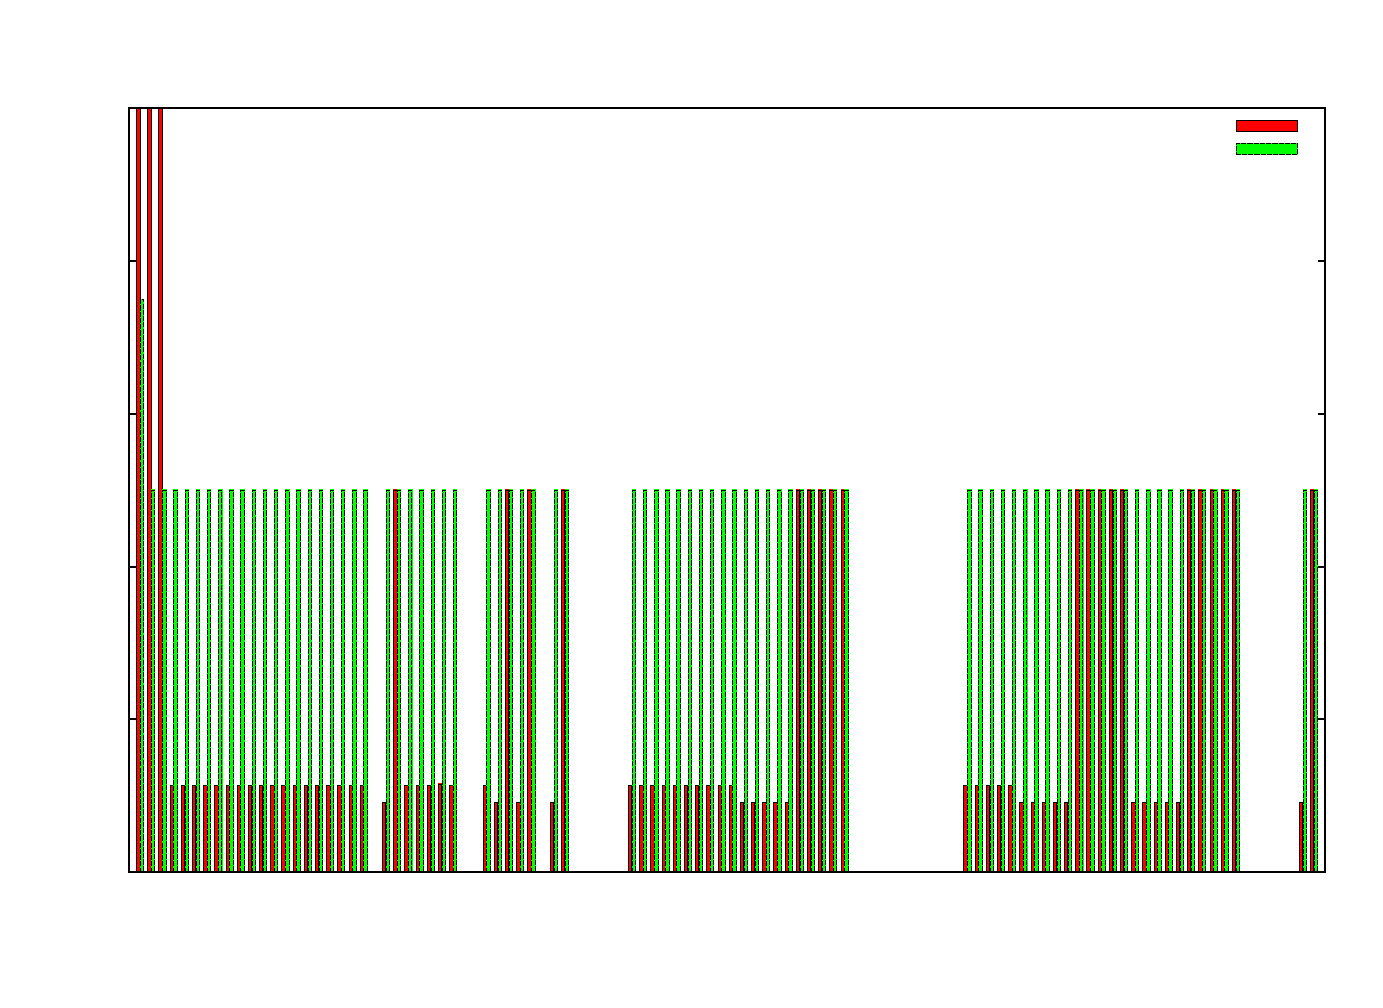
\includegraphics{prec}}%
    \gplfronttext
  \end{picture}%
\endgroup
}
\caption{Comparison of Precision}
\label{fig:precision}
\end{sidewaysfigure}

\begin{sidewaysfigure}
\centering
\tiny{% GNUPLOT: LaTeX picture with Postscript
\begingroup
  \makeatletter
  \providecommand\color[2][]{%
    \GenericError{(gnuplot) \space\space\space\@spaces}{%
      Package color not loaded in conjunction with
      terminal option `colourtext'%
    }{See the gnuplot documentation for explanation.%
    }{Either use 'blacktext' in gnuplot or load the package
      color.sty in LaTeX.}%
    \renewcommand\color[2][]{}%
  }%
  \providecommand\includegraphics[2][]{%
    \GenericError{(gnuplot) \space\space\space\@spaces}{%
      Package graphicx or graphics not loaded%
    }{See the gnuplot documentation for explanation.%
    }{The gnuplot epslatex terminal needs graphicx.sty or graphics.sty.}%
    \renewcommand\includegraphics[2][]{}%
  }%
  \providecommand\rotatebox[2]{#2}%
  \@ifundefined{ifGPcolor}{%
    \newif\ifGPcolor
    \GPcolortrue
  }{}%
  \@ifundefined{ifGPblacktext}{%
    \newif\ifGPblacktext
    \GPblacktexttrue
  }{}%
  % define a \g@addto@macro without @ in the name:
  \let\gplgaddtomacro\g@addto@macro
  % define empty templates for all commands taking text:
  \gdef\gplbacktext{}%
  \gdef\gplfronttext{}%
  \makeatother
  \ifGPblacktext
    % no textcolor at all
    \def\colorrgb#1{}%
    \def\colorgray#1{}%
  \else
    % gray or color?
    \ifGPcolor
      \def\colorrgb#1{\color[rgb]{#1}}%
      \def\colorgray#1{\color[gray]{#1}}%
      \expandafter\def\csname LTw\endcsname{\color{white}}%
      \expandafter\def\csname LTb\endcsname{\color{black}}%
      \expandafter\def\csname LTa\endcsname{\color{black}}%
      \expandafter\def\csname LT0\endcsname{\color[rgb]{1,0,0}}%
      \expandafter\def\csname LT1\endcsname{\color[rgb]{0,1,0}}%
      \expandafter\def\csname LT2\endcsname{\color[rgb]{0,0,1}}%
      \expandafter\def\csname LT3\endcsname{\color[rgb]{1,0,1}}%
      \expandafter\def\csname LT4\endcsname{\color[rgb]{0,1,1}}%
      \expandafter\def\csname LT5\endcsname{\color[rgb]{1,1,0}}%
      \expandafter\def\csname LT6\endcsname{\color[rgb]{0,0,0}}%
      \expandafter\def\csname LT7\endcsname{\color[rgb]{1,0.3,0}}%
      \expandafter\def\csname LT8\endcsname{\color[rgb]{0.5,0.5,0.5}}%
    \else
      % gray
      \def\colorrgb#1{\color{black}}%
      \def\colorgray#1{\color[gray]{#1}}%
      \expandafter\def\csname LTw\endcsname{\color{white}}%
      \expandafter\def\csname LTb\endcsname{\color{black}}%
      \expandafter\def\csname LTa\endcsname{\color{black}}%
      \expandafter\def\csname LT0\endcsname{\color{black}}%
      \expandafter\def\csname LT1\endcsname{\color{black}}%
      \expandafter\def\csname LT2\endcsname{\color{black}}%
      \expandafter\def\csname LT3\endcsname{\color{black}}%
      \expandafter\def\csname LT4\endcsname{\color{black}}%
      \expandafter\def\csname LT5\endcsname{\color{black}}%
      \expandafter\def\csname LT6\endcsname{\color{black}}%
      \expandafter\def\csname LT7\endcsname{\color{black}}%
      \expandafter\def\csname LT8\endcsname{\color{black}}%
    \fi
  \fi
  \setlength{\unitlength}{0.0500bp}%
  \begin{picture}(12960.00,9360.00)%
    \gplgaddtomacro\gplbacktext{%
      \csname LTb\endcsname%
      \put(1078,1144){\makebox(0,0)[r]{\strut{} 0}}%
      \put(1078,2611){\makebox(0,0)[r]{\strut{} 0.05}}%
      \put(1078,4078){\makebox(0,0)[r]{\strut{} 0.1}}%
      \put(1078,5545){\makebox(0,0)[r]{\strut{} 0.15}}%
      \put(1078,7012){\makebox(0,0)[r]{\strut{} 0.2}}%
      \put(1078,8479){\makebox(0,0)[r]{\strut{} 0.25}}%
      \put(1316,1078){\rotatebox{-90}{\makebox(0,0)[l]{\strut{}101}}}%
      \put(1422,1078){\rotatebox{-90}{\makebox(0,0)[l]{\strut{}103}}}%
      \put(1528,1078){\rotatebox{-90}{\makebox(0,0)[l]{\strut{}104}}}%
      \put(1634,1078){\rotatebox{-90}{\makebox(0,0)[l]{\strut{}201}}}%
      \put(1741,1078){\rotatebox{-90}{\makebox(0,0)[l]{\strut{}201-2}}}%
      \put(1847,1078){\rotatebox{-90}{\makebox(0,0)[l]{\strut{}201-4}}}%
      \put(1953,1078){\rotatebox{-90}{\makebox(0,0)[l]{\strut{}201-6}}}%
      \put(2059,1078){\rotatebox{-90}{\makebox(0,0)[l]{\strut{}201-8}}}%
      \put(2165,1078){\rotatebox{-90}{\makebox(0,0)[l]{\strut{}202}}}%
      \put(2271,1078){\rotatebox{-90}{\makebox(0,0)[l]{\strut{}202-2}}}%
      \put(2377,1078){\rotatebox{-90}{\makebox(0,0)[l]{\strut{}202-4}}}%
      \put(2483,1078){\rotatebox{-90}{\makebox(0,0)[l]{\strut{}202-6}}}%
      \put(2589,1078){\rotatebox{-90}{\makebox(0,0)[l]{\strut{}202-8}}}%
      \put(2695,1078){\rotatebox{-90}{\makebox(0,0)[l]{\strut{}203}}}%
      \put(2802,1078){\rotatebox{-90}{\makebox(0,0)[l]{\strut{}204}}}%
      \put(2908,1078){\rotatebox{-90}{\makebox(0,0)[l]{\strut{}205}}}%
      \put(3014,1078){\rotatebox{-90}{\makebox(0,0)[l]{\strut{}206}}}%
      \put(3120,1078){\rotatebox{-90}{\makebox(0,0)[l]{\strut{}207}}}%
      \put(3226,1078){\rotatebox{-90}{\makebox(0,0)[l]{\strut{}208}}}%
      \put(3332,1078){\rotatebox{-90}{\makebox(0,0)[l]{\strut{}209}}}%
      \put(3438,1078){\rotatebox{-90}{\makebox(0,0)[l]{\strut{}210}}}%
      \put(3544,1078){\rotatebox{-90}{\makebox(0,0)[l]{\strut{}221}}}%
      \put(3650,1078){\rotatebox{-90}{\makebox(0,0)[l]{\strut{}222}}}%
      \put(3756,1078){\rotatebox{-90}{\makebox(0,0)[l]{\strut{}223}}}%
      \put(3863,1078){\rotatebox{-90}{\makebox(0,0)[l]{\strut{}224}}}%
      \put(3969,1078){\rotatebox{-90}{\makebox(0,0)[l]{\strut{}225}}}%
      \put(4075,1078){\rotatebox{-90}{\makebox(0,0)[l]{\strut{}228}}}%
      \put(4181,1078){\rotatebox{-90}{\makebox(0,0)[l]{\strut{}230}}}%
      \put(4287,1078){\rotatebox{-90}{\makebox(0,0)[l]{\strut{}231}}}%
      \put(4393,1078){\rotatebox{-90}{\makebox(0,0)[l]{\strut{}232}}}%
      \put(4499,1078){\rotatebox{-90}{\makebox(0,0)[l]{\strut{}233}}}%
      \put(4605,1078){\rotatebox{-90}{\makebox(0,0)[l]{\strut{}236}}}%
      \put(4711,1078){\rotatebox{-90}{\makebox(0,0)[l]{\strut{}237}}}%
      \put(4817,1078){\rotatebox{-90}{\makebox(0,0)[l]{\strut{}238}}}%
      \put(4924,1078){\rotatebox{-90}{\makebox(0,0)[l]{\strut{}239}}}%
      \put(5030,1078){\rotatebox{-90}{\makebox(0,0)[l]{\strut{}240}}}%
      \put(5136,1078){\rotatebox{-90}{\makebox(0,0)[l]{\strut{}241}}}%
      \put(5242,1078){\rotatebox{-90}{\makebox(0,0)[l]{\strut{}246}}}%
      \put(5348,1078){\rotatebox{-90}{\makebox(0,0)[l]{\strut{}247}}}%
      \put(5454,1078){\rotatebox{-90}{\makebox(0,0)[l]{\strut{}248}}}%
      \put(5560,1078){\rotatebox{-90}{\makebox(0,0)[l]{\strut{}248-2}}}%
      \put(5666,1078){\rotatebox{-90}{\makebox(0,0)[l]{\strut{}248-4}}}%
      \put(5772,1078){\rotatebox{-90}{\makebox(0,0)[l]{\strut{}248-6}}}%
      \put(5879,1078){\rotatebox{-90}{\makebox(0,0)[l]{\strut{}248-8}}}%
      \put(5985,1078){\rotatebox{-90}{\makebox(0,0)[l]{\strut{}249}}}%
      \put(6091,1078){\rotatebox{-90}{\makebox(0,0)[l]{\strut{}249-2}}}%
      \put(6197,1078){\rotatebox{-90}{\makebox(0,0)[l]{\strut{}249-4}}}%
      \put(6303,1078){\rotatebox{-90}{\makebox(0,0)[l]{\strut{}249-6}}}%
      \put(6409,1078){\rotatebox{-90}{\makebox(0,0)[l]{\strut{}249-8}}}%
      \put(6515,1078){\rotatebox{-90}{\makebox(0,0)[l]{\strut{}250}}}%
      \put(6621,1078){\rotatebox{-90}{\makebox(0,0)[l]{\strut{}250-2}}}%
      \put(6727,1078){\rotatebox{-90}{\makebox(0,0)[l]{\strut{}250-4}}}%
      \put(6833,1078){\rotatebox{-90}{\makebox(0,0)[l]{\strut{}250-6}}}%
      \put(6940,1078){\rotatebox{-90}{\makebox(0,0)[l]{\strut{}250-8}}}%
      \put(7046,1078){\rotatebox{-90}{\makebox(0,0)[l]{\strut{}251}}}%
      \put(7152,1078){\rotatebox{-90}{\makebox(0,0)[l]{\strut{}251-2}}}%
      \put(7258,1078){\rotatebox{-90}{\makebox(0,0)[l]{\strut{}251-4}}}%
      \put(7364,1078){\rotatebox{-90}{\makebox(0,0)[l]{\strut{}251-6}}}%
      \put(7470,1078){\rotatebox{-90}{\makebox(0,0)[l]{\strut{}251-8}}}%
      \put(7576,1078){\rotatebox{-90}{\makebox(0,0)[l]{\strut{}252}}}%
      \put(7682,1078){\rotatebox{-90}{\makebox(0,0)[l]{\strut{}252-2}}}%
      \put(7788,1078){\rotatebox{-90}{\makebox(0,0)[l]{\strut{}252-4}}}%
      \put(7894,1078){\rotatebox{-90}{\makebox(0,0)[l]{\strut{}252-6}}}%
      \put(8001,1078){\rotatebox{-90}{\makebox(0,0)[l]{\strut{}252-8}}}%
      \put(8107,1078){\rotatebox{-90}{\makebox(0,0)[l]{\strut{}253}}}%
      \put(8213,1078){\rotatebox{-90}{\makebox(0,0)[l]{\strut{}253-2}}}%
      \put(8319,1078){\rotatebox{-90}{\makebox(0,0)[l]{\strut{}253-4}}}%
      \put(8425,1078){\rotatebox{-90}{\makebox(0,0)[l]{\strut{}253-6}}}%
      \put(8531,1078){\rotatebox{-90}{\makebox(0,0)[l]{\strut{}253-8}}}%
      \put(8637,1078){\rotatebox{-90}{\makebox(0,0)[l]{\strut{}254}}}%
      \put(8743,1078){\rotatebox{-90}{\makebox(0,0)[l]{\strut{}254-2}}}%
      \put(8849,1078){\rotatebox{-90}{\makebox(0,0)[l]{\strut{}254-4}}}%
      \put(8956,1078){\rotatebox{-90}{\makebox(0,0)[l]{\strut{}254-6}}}%
      \put(9062,1078){\rotatebox{-90}{\makebox(0,0)[l]{\strut{}254-8}}}%
      \put(9168,1078){\rotatebox{-90}{\makebox(0,0)[l]{\strut{}257}}}%
      \put(9274,1078){\rotatebox{-90}{\makebox(0,0)[l]{\strut{}257-2}}}%
      \put(9380,1078){\rotatebox{-90}{\makebox(0,0)[l]{\strut{}257-4}}}%
      \put(9486,1078){\rotatebox{-90}{\makebox(0,0)[l]{\strut{}257-6}}}%
      \put(9592,1078){\rotatebox{-90}{\makebox(0,0)[l]{\strut{}257-8}}}%
      \put(9698,1078){\rotatebox{-90}{\makebox(0,0)[l]{\strut{}258}}}%
      \put(9804,1078){\rotatebox{-90}{\makebox(0,0)[l]{\strut{}258-2}}}%
      \put(9910,1078){\rotatebox{-90}{\makebox(0,0)[l]{\strut{}258-4}}}%
      \put(10017,1078){\rotatebox{-90}{\makebox(0,0)[l]{\strut{}258-6}}}%
      \put(10123,1078){\rotatebox{-90}{\makebox(0,0)[l]{\strut{}258-8}}}%
      \put(10229,1078){\rotatebox{-90}{\makebox(0,0)[l]{\strut{}259}}}%
      \put(10335,1078){\rotatebox{-90}{\makebox(0,0)[l]{\strut{}259-2}}}%
      \put(10441,1078){\rotatebox{-90}{\makebox(0,0)[l]{\strut{}259-4}}}%
      \put(10547,1078){\rotatebox{-90}{\makebox(0,0)[l]{\strut{}259-6}}}%
      \put(10653,1078){\rotatebox{-90}{\makebox(0,0)[l]{\strut{}259-8}}}%
      \put(10759,1078){\rotatebox{-90}{\makebox(0,0)[l]{\strut{}260}}}%
      \put(10865,1078){\rotatebox{-90}{\makebox(0,0)[l]{\strut{}260-2}}}%
      \put(10971,1078){\rotatebox{-90}{\makebox(0,0)[l]{\strut{}260-4}}}%
      \put(11078,1078){\rotatebox{-90}{\makebox(0,0)[l]{\strut{}260-6}}}%
      \put(11184,1078){\rotatebox{-90}{\makebox(0,0)[l]{\strut{}260-8}}}%
      \put(11290,1078){\rotatebox{-90}{\makebox(0,0)[l]{\strut{}261}}}%
      \put(11396,1078){\rotatebox{-90}{\makebox(0,0)[l]{\strut{}261-2}}}%
      \put(11502,1078){\rotatebox{-90}{\makebox(0,0)[l]{\strut{}261-4}}}%
      \put(11608,1078){\rotatebox{-90}{\makebox(0,0)[l]{\strut{}261-6}}}%
      \put(11714,1078){\rotatebox{-90}{\makebox(0,0)[l]{\strut{}261-8}}}%
      \put(11820,1078){\rotatebox{-90}{\makebox(0,0)[l]{\strut{}262}}}%
      \put(11926,1078){\rotatebox{-90}{\makebox(0,0)[l]{\strut{}262-2}}}%
      \put(12032,1078){\rotatebox{-90}{\makebox(0,0)[l]{\strut{}262-4}}}%
      \put(12139,1078){\rotatebox{-90}{\makebox(0,0)[l]{\strut{}262-6}}}%
      \put(12245,1078){\rotatebox{-90}{\makebox(0,0)[l]{\strut{}262-8}}}%
      \put(12351,1078){\rotatebox{-90}{\makebox(0,0)[l]{\strut{}265}}}%
      \put(12457,1078){\rotatebox{-90}{\makebox(0,0)[l]{\strut{}266}}}%
      \put(176,4811){\rotatebox{-270}{\makebox(0,0){\strut{}Recall}}}%
      \put(6886,154){\makebox(0,0){\strut{}Test Number}}%
      \put(6886,9029){\makebox(0,0){\strut{}Similarity Flooding vs Edge Confidence: Recall comparison}}%
      \put(6886,8809){\makebox(0,0){\strut{} OAEI Benchmark 1 suite}}%
    }%
    \gplgaddtomacro\gplfronttext{%
      \csname LTb\endcsname%
      \put(11576,8306){\makebox(0,0)[r]{\strut{}Edge Conf}}%
      \csname LTb\endcsname%
      \put(11576,8086){\makebox(0,0)[r]{\strut{}Sim Flood}}%
    }%
    \gplbacktext
    \put(0,0){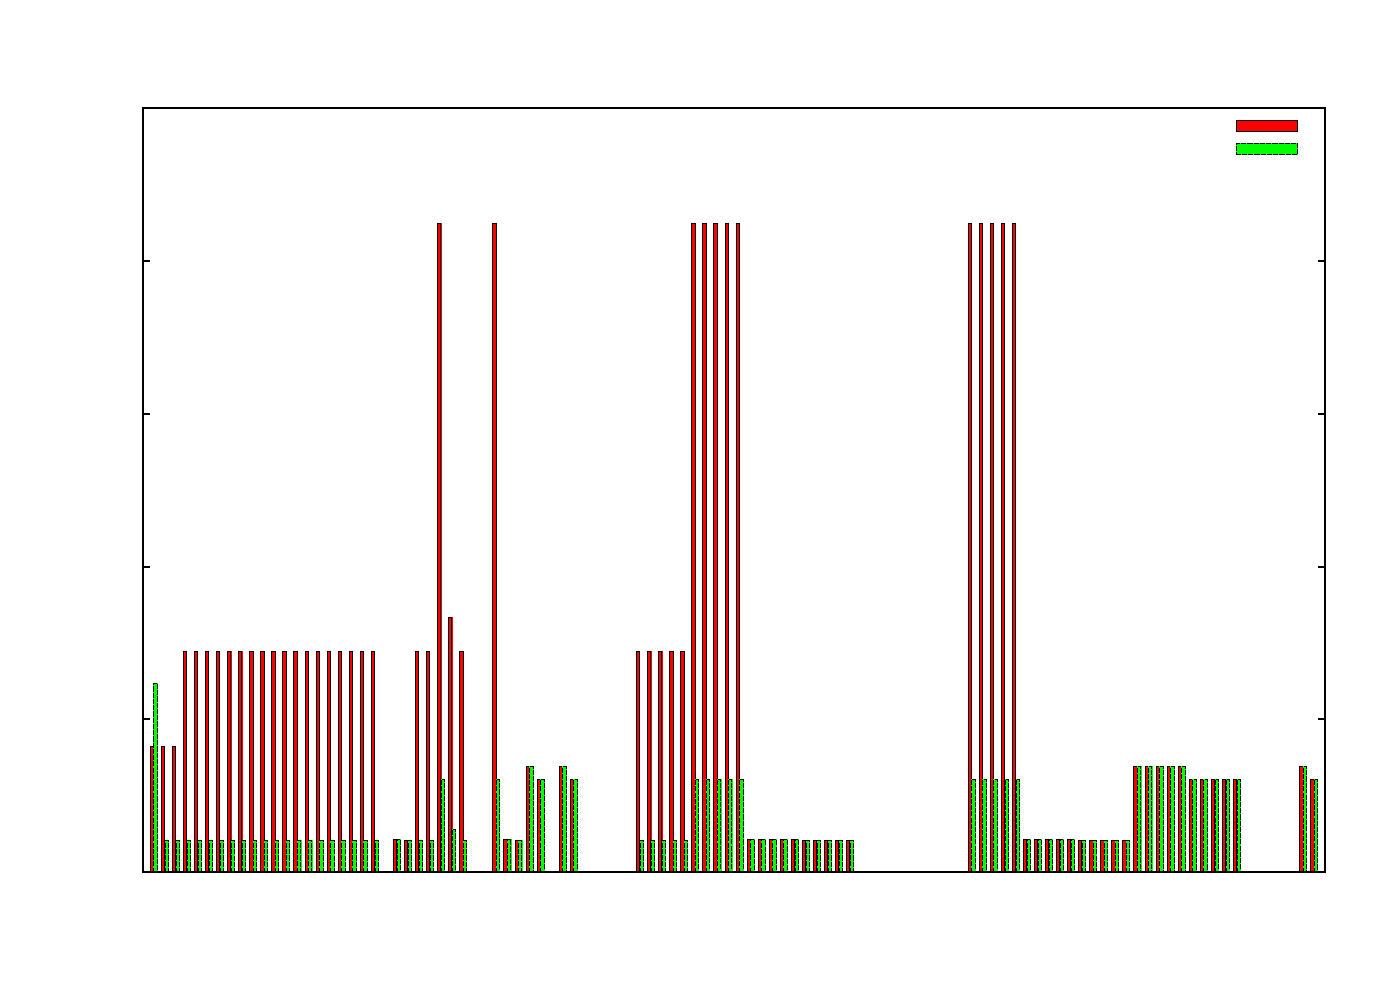
\includegraphics{recall}}%
    \gplfronttext
  \end{picture}%
\endgroup
}
\caption{Comparison of Recall}
\label{fig:recall}
\end{sidewaysfigure}

\begin{sidewaysfigure}
\centering
\tiny{% GNUPLOT: LaTeX picture with Postscript
\begingroup
  \makeatletter
  \providecommand\color[2][]{%
    \GenericError{(gnuplot) \space\space\space\@spaces}{%
      Package color not loaded in conjunction with
      terminal option `colourtext'%
    }{See the gnuplot documentation for explanation.%
    }{Either use 'blacktext' in gnuplot or load the package
      color.sty in LaTeX.}%
    \renewcommand\color[2][]{}%
  }%
  \providecommand\includegraphics[2][]{%
    \GenericError{(gnuplot) \space\space\space\@spaces}{%
      Package graphicx or graphics not loaded%
    }{See the gnuplot documentation for explanation.%
    }{The gnuplot epslatex terminal needs graphicx.sty or graphics.sty.}%
    \renewcommand\includegraphics[2][]{}%
  }%
  \providecommand\rotatebox[2]{#2}%
  \@ifundefined{ifGPcolor}{%
    \newif\ifGPcolor
    \GPcolortrue
  }{}%
  \@ifundefined{ifGPblacktext}{%
    \newif\ifGPblacktext
    \GPblacktexttrue
  }{}%
  % define a \g@addto@macro without @ in the name:
  \let\gplgaddtomacro\g@addto@macro
  % define empty templates for all commands taking text:
  \gdef\gplbacktext{}%
  \gdef\gplfronttext{}%
  \makeatother
  \ifGPblacktext
    % no textcolor at all
    \def\colorrgb#1{}%
    \def\colorgray#1{}%
  \else
    % gray or color?
    \ifGPcolor
      \def\colorrgb#1{\color[rgb]{#1}}%
      \def\colorgray#1{\color[gray]{#1}}%
      \expandafter\def\csname LTw\endcsname{\color{white}}%
      \expandafter\def\csname LTb\endcsname{\color{black}}%
      \expandafter\def\csname LTa\endcsname{\color{black}}%
      \expandafter\def\csname LT0\endcsname{\color[rgb]{1,0,0}}%
      \expandafter\def\csname LT1\endcsname{\color[rgb]{0,1,0}}%
      \expandafter\def\csname LT2\endcsname{\color[rgb]{0,0,1}}%
      \expandafter\def\csname LT3\endcsname{\color[rgb]{1,0,1}}%
      \expandafter\def\csname LT4\endcsname{\color[rgb]{0,1,1}}%
      \expandafter\def\csname LT5\endcsname{\color[rgb]{1,1,0}}%
      \expandafter\def\csname LT6\endcsname{\color[rgb]{0,0,0}}%
      \expandafter\def\csname LT7\endcsname{\color[rgb]{1,0.3,0}}%
      \expandafter\def\csname LT8\endcsname{\color[rgb]{0.5,0.5,0.5}}%
    \else
      % gray
      \def\colorrgb#1{\color{black}}%
      \def\colorgray#1{\color[gray]{#1}}%
      \expandafter\def\csname LTw\endcsname{\color{white}}%
      \expandafter\def\csname LTb\endcsname{\color{black}}%
      \expandafter\def\csname LTa\endcsname{\color{black}}%
      \expandafter\def\csname LT0\endcsname{\color{black}}%
      \expandafter\def\csname LT1\endcsname{\color{black}}%
      \expandafter\def\csname LT2\endcsname{\color{black}}%
      \expandafter\def\csname LT3\endcsname{\color{black}}%
      \expandafter\def\csname LT4\endcsname{\color{black}}%
      \expandafter\def\csname LT5\endcsname{\color{black}}%
      \expandafter\def\csname LT6\endcsname{\color{black}}%
      \expandafter\def\csname LT7\endcsname{\color{black}}%
      \expandafter\def\csname LT8\endcsname{\color{black}}%
    \fi
  \fi
  \setlength{\unitlength}{0.0500bp}%
  \begin{picture}(12960.00,9360.00)%
    \gplgaddtomacro\gplbacktext{%
      \csname LTb\endcsname%
      \put(1078,1144){\makebox(0,0)[r]{\strut{} 0}}%
      \put(1078,2061){\makebox(0,0)[r]{\strut{} 0.02}}%
      \put(1078,2978){\makebox(0,0)[r]{\strut{} 0.04}}%
      \put(1078,3895){\makebox(0,0)[r]{\strut{} 0.06}}%
      \put(1078,4812){\makebox(0,0)[r]{\strut{} 0.08}}%
      \put(1078,5728){\makebox(0,0)[r]{\strut{} 0.1}}%
      \put(1078,6645){\makebox(0,0)[r]{\strut{} 0.12}}%
      \put(1078,7562){\makebox(0,0)[r]{\strut{} 0.14}}%
      \put(1078,8479){\makebox(0,0)[r]{\strut{} 0.16}}%
      \put(1316,1078){\rotatebox{-90}{\makebox(0,0)[l]{\strut{}101}}}%
      \put(1422,1078){\rotatebox{-90}{\makebox(0,0)[l]{\strut{}103}}}%
      \put(1528,1078){\rotatebox{-90}{\makebox(0,0)[l]{\strut{}104}}}%
      \put(1634,1078){\rotatebox{-90}{\makebox(0,0)[l]{\strut{}201}}}%
      \put(1741,1078){\rotatebox{-90}{\makebox(0,0)[l]{\strut{}201-2}}}%
      \put(1847,1078){\rotatebox{-90}{\makebox(0,0)[l]{\strut{}201-4}}}%
      \put(1953,1078){\rotatebox{-90}{\makebox(0,0)[l]{\strut{}201-6}}}%
      \put(2059,1078){\rotatebox{-90}{\makebox(0,0)[l]{\strut{}201-8}}}%
      \put(2165,1078){\rotatebox{-90}{\makebox(0,0)[l]{\strut{}202}}}%
      \put(2271,1078){\rotatebox{-90}{\makebox(0,0)[l]{\strut{}202-2}}}%
      \put(2377,1078){\rotatebox{-90}{\makebox(0,0)[l]{\strut{}202-4}}}%
      \put(2483,1078){\rotatebox{-90}{\makebox(0,0)[l]{\strut{}202-6}}}%
      \put(2589,1078){\rotatebox{-90}{\makebox(0,0)[l]{\strut{}202-8}}}%
      \put(2695,1078){\rotatebox{-90}{\makebox(0,0)[l]{\strut{}203}}}%
      \put(2802,1078){\rotatebox{-90}{\makebox(0,0)[l]{\strut{}204}}}%
      \put(2908,1078){\rotatebox{-90}{\makebox(0,0)[l]{\strut{}205}}}%
      \put(3014,1078){\rotatebox{-90}{\makebox(0,0)[l]{\strut{}206}}}%
      \put(3120,1078){\rotatebox{-90}{\makebox(0,0)[l]{\strut{}207}}}%
      \put(3226,1078){\rotatebox{-90}{\makebox(0,0)[l]{\strut{}208}}}%
      \put(3332,1078){\rotatebox{-90}{\makebox(0,0)[l]{\strut{}209}}}%
      \put(3438,1078){\rotatebox{-90}{\makebox(0,0)[l]{\strut{}210}}}%
      \put(3544,1078){\rotatebox{-90}{\makebox(0,0)[l]{\strut{}221}}}%
      \put(3650,1078){\rotatebox{-90}{\makebox(0,0)[l]{\strut{}222}}}%
      \put(3756,1078){\rotatebox{-90}{\makebox(0,0)[l]{\strut{}223}}}%
      \put(3863,1078){\rotatebox{-90}{\makebox(0,0)[l]{\strut{}224}}}%
      \put(3969,1078){\rotatebox{-90}{\makebox(0,0)[l]{\strut{}225}}}%
      \put(4075,1078){\rotatebox{-90}{\makebox(0,0)[l]{\strut{}228}}}%
      \put(4181,1078){\rotatebox{-90}{\makebox(0,0)[l]{\strut{}230}}}%
      \put(4287,1078){\rotatebox{-90}{\makebox(0,0)[l]{\strut{}231}}}%
      \put(4393,1078){\rotatebox{-90}{\makebox(0,0)[l]{\strut{}232}}}%
      \put(4499,1078){\rotatebox{-90}{\makebox(0,0)[l]{\strut{}233}}}%
      \put(4605,1078){\rotatebox{-90}{\makebox(0,0)[l]{\strut{}236}}}%
      \put(4711,1078){\rotatebox{-90}{\makebox(0,0)[l]{\strut{}237}}}%
      \put(4817,1078){\rotatebox{-90}{\makebox(0,0)[l]{\strut{}238}}}%
      \put(4924,1078){\rotatebox{-90}{\makebox(0,0)[l]{\strut{}239}}}%
      \put(5030,1078){\rotatebox{-90}{\makebox(0,0)[l]{\strut{}240}}}%
      \put(5136,1078){\rotatebox{-90}{\makebox(0,0)[l]{\strut{}241}}}%
      \put(5242,1078){\rotatebox{-90}{\makebox(0,0)[l]{\strut{}246}}}%
      \put(5348,1078){\rotatebox{-90}{\makebox(0,0)[l]{\strut{}247}}}%
      \put(5454,1078){\rotatebox{-90}{\makebox(0,0)[l]{\strut{}248}}}%
      \put(5560,1078){\rotatebox{-90}{\makebox(0,0)[l]{\strut{}248-2}}}%
      \put(5666,1078){\rotatebox{-90}{\makebox(0,0)[l]{\strut{}248-4}}}%
      \put(5772,1078){\rotatebox{-90}{\makebox(0,0)[l]{\strut{}248-6}}}%
      \put(5879,1078){\rotatebox{-90}{\makebox(0,0)[l]{\strut{}248-8}}}%
      \put(5985,1078){\rotatebox{-90}{\makebox(0,0)[l]{\strut{}249}}}%
      \put(6091,1078){\rotatebox{-90}{\makebox(0,0)[l]{\strut{}249-2}}}%
      \put(6197,1078){\rotatebox{-90}{\makebox(0,0)[l]{\strut{}249-4}}}%
      \put(6303,1078){\rotatebox{-90}{\makebox(0,0)[l]{\strut{}249-6}}}%
      \put(6409,1078){\rotatebox{-90}{\makebox(0,0)[l]{\strut{}249-8}}}%
      \put(6515,1078){\rotatebox{-90}{\makebox(0,0)[l]{\strut{}250}}}%
      \put(6621,1078){\rotatebox{-90}{\makebox(0,0)[l]{\strut{}250-2}}}%
      \put(6727,1078){\rotatebox{-90}{\makebox(0,0)[l]{\strut{}250-4}}}%
      \put(6833,1078){\rotatebox{-90}{\makebox(0,0)[l]{\strut{}250-6}}}%
      \put(6940,1078){\rotatebox{-90}{\makebox(0,0)[l]{\strut{}250-8}}}%
      \put(7046,1078){\rotatebox{-90}{\makebox(0,0)[l]{\strut{}251}}}%
      \put(7152,1078){\rotatebox{-90}{\makebox(0,0)[l]{\strut{}251-2}}}%
      \put(7258,1078){\rotatebox{-90}{\makebox(0,0)[l]{\strut{}251-4}}}%
      \put(7364,1078){\rotatebox{-90}{\makebox(0,0)[l]{\strut{}251-6}}}%
      \put(7470,1078){\rotatebox{-90}{\makebox(0,0)[l]{\strut{}251-8}}}%
      \put(7576,1078){\rotatebox{-90}{\makebox(0,0)[l]{\strut{}252}}}%
      \put(7682,1078){\rotatebox{-90}{\makebox(0,0)[l]{\strut{}252-2}}}%
      \put(7788,1078){\rotatebox{-90}{\makebox(0,0)[l]{\strut{}252-4}}}%
      \put(7894,1078){\rotatebox{-90}{\makebox(0,0)[l]{\strut{}252-6}}}%
      \put(8001,1078){\rotatebox{-90}{\makebox(0,0)[l]{\strut{}252-8}}}%
      \put(8107,1078){\rotatebox{-90}{\makebox(0,0)[l]{\strut{}253}}}%
      \put(8213,1078){\rotatebox{-90}{\makebox(0,0)[l]{\strut{}253-2}}}%
      \put(8319,1078){\rotatebox{-90}{\makebox(0,0)[l]{\strut{}253-4}}}%
      \put(8425,1078){\rotatebox{-90}{\makebox(0,0)[l]{\strut{}253-6}}}%
      \put(8531,1078){\rotatebox{-90}{\makebox(0,0)[l]{\strut{}253-8}}}%
      \put(8637,1078){\rotatebox{-90}{\makebox(0,0)[l]{\strut{}254}}}%
      \put(8743,1078){\rotatebox{-90}{\makebox(0,0)[l]{\strut{}254-2}}}%
      \put(8849,1078){\rotatebox{-90}{\makebox(0,0)[l]{\strut{}254-4}}}%
      \put(8956,1078){\rotatebox{-90}{\makebox(0,0)[l]{\strut{}254-6}}}%
      \put(9062,1078){\rotatebox{-90}{\makebox(0,0)[l]{\strut{}254-8}}}%
      \put(9168,1078){\rotatebox{-90}{\makebox(0,0)[l]{\strut{}257}}}%
      \put(9274,1078){\rotatebox{-90}{\makebox(0,0)[l]{\strut{}257-2}}}%
      \put(9380,1078){\rotatebox{-90}{\makebox(0,0)[l]{\strut{}257-4}}}%
      \put(9486,1078){\rotatebox{-90}{\makebox(0,0)[l]{\strut{}257-6}}}%
      \put(9592,1078){\rotatebox{-90}{\makebox(0,0)[l]{\strut{}257-8}}}%
      \put(9698,1078){\rotatebox{-90}{\makebox(0,0)[l]{\strut{}258}}}%
      \put(9804,1078){\rotatebox{-90}{\makebox(0,0)[l]{\strut{}258-2}}}%
      \put(9910,1078){\rotatebox{-90}{\makebox(0,0)[l]{\strut{}258-4}}}%
      \put(10017,1078){\rotatebox{-90}{\makebox(0,0)[l]{\strut{}258-6}}}%
      \put(10123,1078){\rotatebox{-90}{\makebox(0,0)[l]{\strut{}258-8}}}%
      \put(10229,1078){\rotatebox{-90}{\makebox(0,0)[l]{\strut{}259}}}%
      \put(10335,1078){\rotatebox{-90}{\makebox(0,0)[l]{\strut{}259-2}}}%
      \put(10441,1078){\rotatebox{-90}{\makebox(0,0)[l]{\strut{}259-4}}}%
      \put(10547,1078){\rotatebox{-90}{\makebox(0,0)[l]{\strut{}259-6}}}%
      \put(10653,1078){\rotatebox{-90}{\makebox(0,0)[l]{\strut{}259-8}}}%
      \put(10759,1078){\rotatebox{-90}{\makebox(0,0)[l]{\strut{}260}}}%
      \put(10865,1078){\rotatebox{-90}{\makebox(0,0)[l]{\strut{}260-2}}}%
      \put(10971,1078){\rotatebox{-90}{\makebox(0,0)[l]{\strut{}260-4}}}%
      \put(11078,1078){\rotatebox{-90}{\makebox(0,0)[l]{\strut{}260-6}}}%
      \put(11184,1078){\rotatebox{-90}{\makebox(0,0)[l]{\strut{}260-8}}}%
      \put(11290,1078){\rotatebox{-90}{\makebox(0,0)[l]{\strut{}261}}}%
      \put(11396,1078){\rotatebox{-90}{\makebox(0,0)[l]{\strut{}261-2}}}%
      \put(11502,1078){\rotatebox{-90}{\makebox(0,0)[l]{\strut{}261-4}}}%
      \put(11608,1078){\rotatebox{-90}{\makebox(0,0)[l]{\strut{}261-6}}}%
      \put(11714,1078){\rotatebox{-90}{\makebox(0,0)[l]{\strut{}261-8}}}%
      \put(11820,1078){\rotatebox{-90}{\makebox(0,0)[l]{\strut{}262}}}%
      \put(11926,1078){\rotatebox{-90}{\makebox(0,0)[l]{\strut{}262-2}}}%
      \put(12032,1078){\rotatebox{-90}{\makebox(0,0)[l]{\strut{}262-4}}}%
      \put(12139,1078){\rotatebox{-90}{\makebox(0,0)[l]{\strut{}262-6}}}%
      \put(12245,1078){\rotatebox{-90}{\makebox(0,0)[l]{\strut{}262-8}}}%
      \put(12351,1078){\rotatebox{-90}{\makebox(0,0)[l]{\strut{}265}}}%
      \put(12457,1078){\rotatebox{-90}{\makebox(0,0)[l]{\strut{}266}}}%
      \put(176,4811){\rotatebox{-270}{\makebox(0,0){\strut{}F-measure}}}%
      \put(6886,154){\makebox(0,0){\strut{}Test Number}}%
      \put(6886,9029){\makebox(0,0){\strut{}Similarity Flooding vs Edge Confidence: F-measure comparison}}%
      \put(6886,8809){\makebox(0,0){\strut{} OAEI Benchmark 1 suite}}%
    }%
    \gplgaddtomacro\gplfronttext{%
      \csname LTb\endcsname%
      \put(11576,8306){\makebox(0,0)[r]{\strut{}Edge Conf}}%
      \csname LTb\endcsname%
      \put(11576,8086){\makebox(0,0)[r]{\strut{}Sim Flood}}%
    }%
    \gplbacktext
    \put(0,0){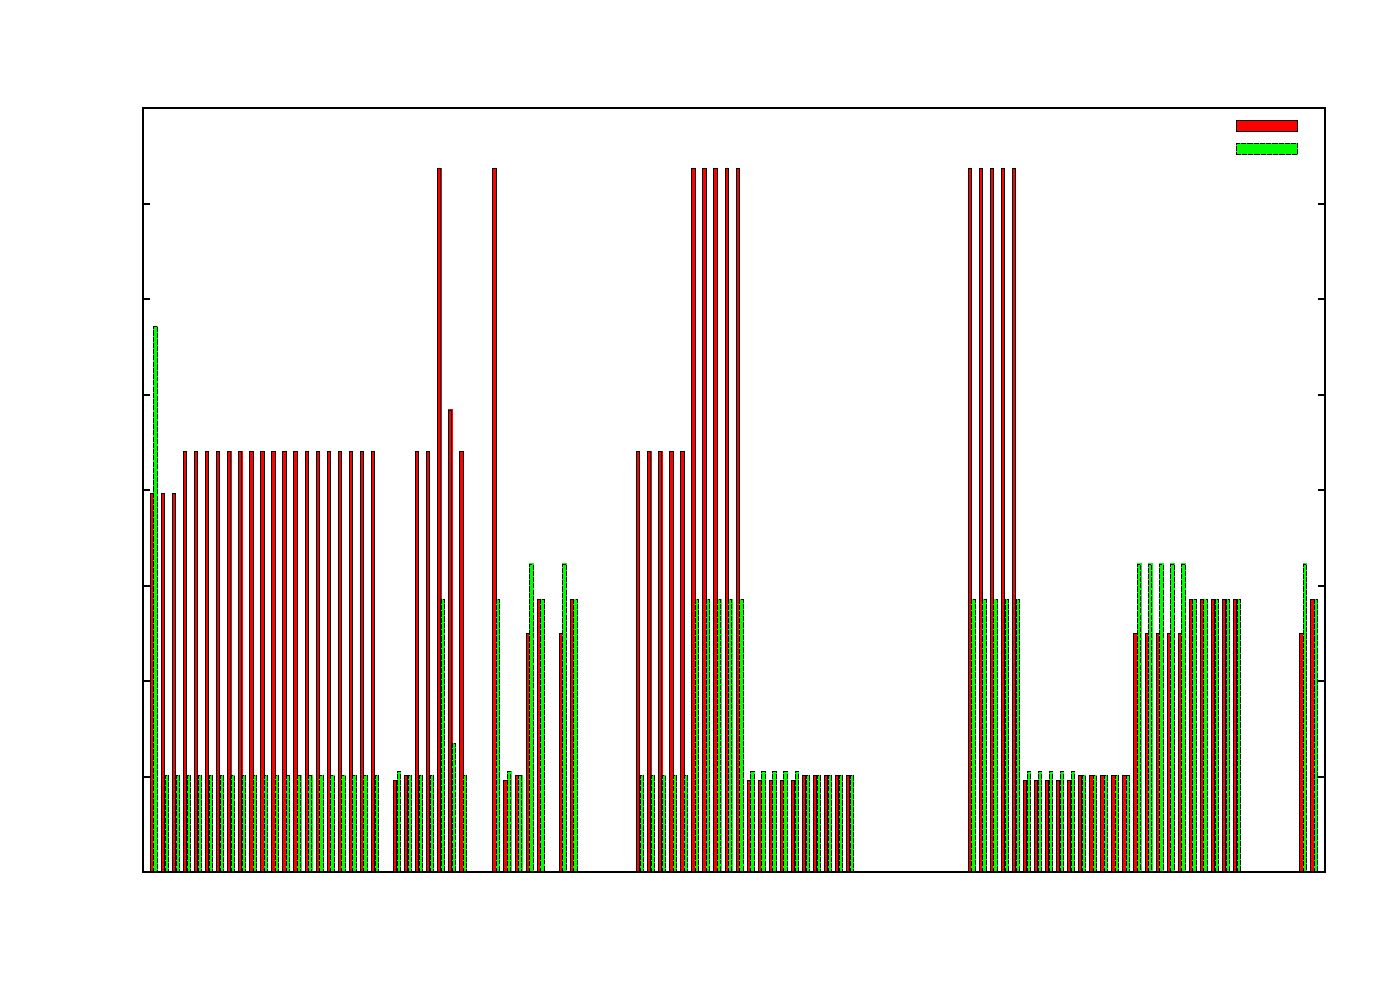
\includegraphics{fmeasure}}%
    \gplfronttext
  \end{picture}%
\endgroup
}
\caption{Comparison of F-measure}
\label{fig:fmeasure}
\end{sidewaysfigure}


\end{document}


